% ===========================================================================
%
%		FEDERICO II THESIS TEMPLATE - ENGLISH
%  					* an example of Chapter 3: tables, figures and software code
%	 
% 		AUTHOR:  		Antonio Esposito (antonio.esposito103@studenti.unina.it)
%		LAST UPDATED:	2017/06/20
%
% ===========================================================================

\chapter{Tables, figures, software code}

The inclusion of tables and figures in a scientific publication follows
certain common and certain specific rules. Tables and figures are not
included inside the text but placed either on dedicated pages or floated
at the top or the bottom of a text page. \LaTeX\ handles floating
figures and tables automatically. Every table and figure must be
numbered and accompanied with a legend. The legend should describe the
contents of the table of figure with enough detail so that the reader
can understand them without studying the text of the publication. Each
table and figure should be refrenced by its number in the text. The
text should summarize the most important conclusions that can be drawn
from the table of figure. The text should be easy to follow and
understand even without seeingf the figures and tables (and on the
contrary, the figures and tables should be easy to understand even
without reading the text). Figures and tables should be referenced
indirectly in the sentences: instead of
\emph{``Table~\ref{tab03:Nejaka} shows that men are on average $9.9$
  kg heavier than women''} we write \emph{``Men are on average $9,9$
  kg heavier than women (see Table~\ref{tab03:Nejaka})}.


%%%%% ===============================================================================
\section{Tables}

\begin{table}[b!]

\centering
%%% The following packages are needed for this example:
%%%   - booktabs (\toprule, \midrule, \bottomrule)
%%%   - dcolumn (column type  D)
%%% Commands \pulrad and \mc defined in BcPrace.tex are used

\begin{tabular}{l@{\hspace{1.5cm}}D{.}{.}{3.2}D{.}{.}{1.2}D{.}{.}{2.3}}
\toprule
 & \mc{} & \mc{\textbf{Std.}} & \mc{} \\
\pulrad{\textbf{Effect}} & \mc{\pulrad{\textbf{Estimate}}} & \mc{\textbf{error}$^a$} & 
\mc{\pulrad{\textbf{P-value}}} \\
\midrule
Intercept     & -10.01 & 1.01 & \mc{---} \\
Gender (male) & 9.89   & 5.98 & 0.098 \\
Height (cm)    & 0.78   & 0.12 & <0.001 \\ 
\bottomrule
\multicolumn{4}{l}{\footnotesize \textit{Note:} 
$^a$ Standard error of the estimator by the Monte Carlo method.}
\end{tabular}

\caption{Maximum likelihood estimates from model M.}\label{tab03:Nejaka}

\end{table}


\textbf{Tables} should be formatted according to the following rules:
\begin{compactitem} %% requires package paralist
\item Avoid vertical lines. Separate the table from the surrounding
  text (even the legend) by stronger horizontal lines. Separate the
  header from the table and different parts of the table from each
  other by thinner horizontal lines. This table format can be obtained
  in \LaTeX\ by loading the package \texttt{booktabs}. If a stronger
  separation of the columns is desired it can be achieved by including
  an additional vertical space. 
\item Do not change the type, format and meaning of the cells in a
  single column (never include means in some cells and percentages in
  other cells of the same column).
\item Do not repeat the same cell contents many times. If the table
  includes the column ``Variance'', which contains the value 0.5 in
  the first ten cells and 1.5 in the next ten cells, delete this
  column and find another way to communicate the value of the
  variance. For example, the table can be divided into two separate
  tables and the variance given in the legend. Or additional rows can
  be included between the parts of the table informing what was the
  variance in the subsequent rows.
\item Numeric columns in the table should be aligned on the decimal
  point. 
\item Tables sometimes include abbreviations that are not used
  elsewhere in the text. These abbreviations should be explained in
  the legend or in notes under the table. These notes can be also used
  to provide more detail on the meaning of selected columns or cells. 
\end{compactitem}




\section{Figures}

Some advice on figures and diagrams:
\begin{compactitem}
\item Create the figure in the same size that will be used in the
  thesis. Excessive magnification or reduction of figures causes poor
  readability.
\item The axes of a graph must be carefully annotated in the same
  language the thesis is written in. Units of measurement (kg,
  minutes, \ldots) should be provided when applicable. When the graph
  plots a function $h(x)$ the axes should be annotated by $x$ a
  $h(x)$. Each axis must have a clearly defined scale (tickmarks, labels).
\item If a two-dimensional scatterplot includes a large number of
  points make sure that the points do not turn into black cloud. If
  the number of points is too large reduce the size of the plotting
  symbol or select a subset of the points. Plots that include
  thousands of points make problems in electronic documents, they
  increase the size too much.
\item If the thesis is to be printed on a black-and-white printer, do
  not use colors. Lines can be distinguished by the type (solid,
  dotted, \ldots), areas can be filled by various shades of grey or 

The meaning of the line types and area shading should be explained in
the legend or directly in the plot.
\end{compactitem}

The command \texttt{{\textbackslash}psfrag} can replace parts of 
\textsf{ps/eps} files (usually annotations in the graphs) by an
arbitrary sequence of \LaTeX\ commands, as the following examples
illustrate. 



\section{Software code}

Software code or computer output (if needed in the thesis) should be
formatted differently from the other text. One option is to use
{\LaTeX} package \texttt{fancyvrb}
(fancy verbatim), which is used to define the environment
\texttt{PCinout} in the master file \texttt{BcPrace.tex}. With this
environment, we can generate the following examples:
\begin{PCinout}
> mean(x)
[1] 158.90
> objekt$mean
[1] 158.90
\end{PCinout}
%$
Smaller font:
\begin{PCinout}[fontsize=\footnotesize]
> mean(x)
[1] 158.90
> objekt$mean
[1] 158.90
\end{PCinout}
%$
No frame:
\begin{PCinout}[frame=none]
> mean(x)
[1] 158.90
> objekt$mean
[1] 158.90
\end{PCinout}
%$
Narrow frame:
\begin{PCinout}[xrightmargin=20em]
> mean(x)
[1] 158.90
> objekt$mean
[1] 158.90
\end{PCinout}
%$


\begin{figure}[p]\centering
\psfrag{x}[c][c]{\textsf{\large horizontal axis ($\mu_1 = 0, \sigma_1^2 = 1$)}}
\psfrag{y}[c][c]{\textsf{\large vertical axis ($\mu_2 = 0, \sigma_2^2 = 1$)}}
\psfrag{Plot}[c][c]{\textsf{\bfseries\Large Scatterplot}}

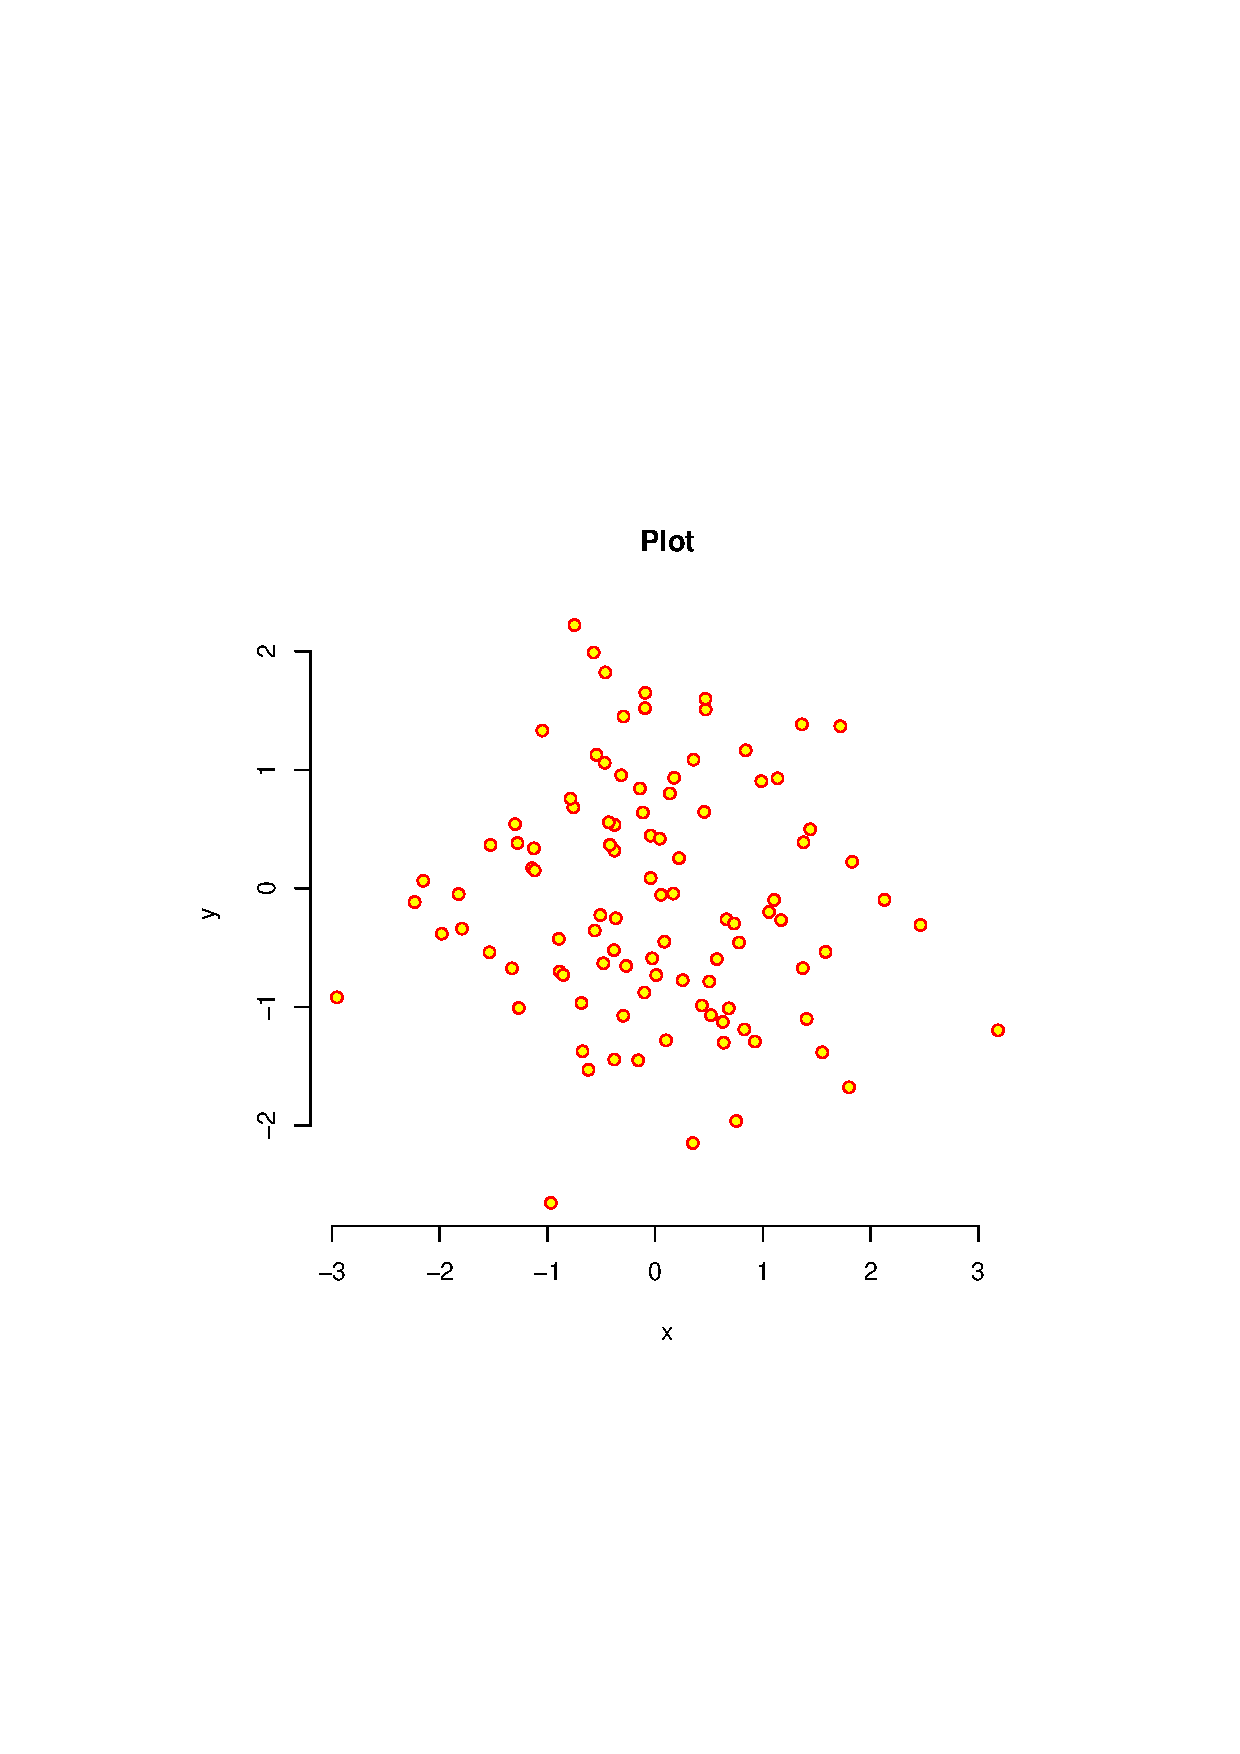
\includegraphics[width=6in, height=6in]{\FIGDIR/obr01}     

\caption{Random sample from distribution $\mathcal{N}_2(\boldsymbol{0},\,I)$.}
\label{obr03:Nvyber}

\end{figure}


\begin{figure}[p]\centering
\psfrag{0.00}[c][c]{\textsf{0{,}00}}  
\psfrag{0.02}[c][c]{\textsf{0{,}02}}  
\psfrag{0.04}[c][c]{\textsf{0{,}04}}
\psfrag{0.06}[c][c]{\textsf{0{,}06}}  
\psfrag{0.08}[c][c]{\textsf{0{,}08}}
\psfrag{m = 100, s = 15}[l][l]{\textsf{\large $\mu = 100,\; \sigma = 15$}}
\psfrag{m = 110, s = 10}[l][l]{\textsf{\large $\mu = 110,\; \sigma = 10$}}
\psfrag{m = 120, s = 5}[l][l]{\textsf{\large $\mu = 120,\; \sigma = 5$}}

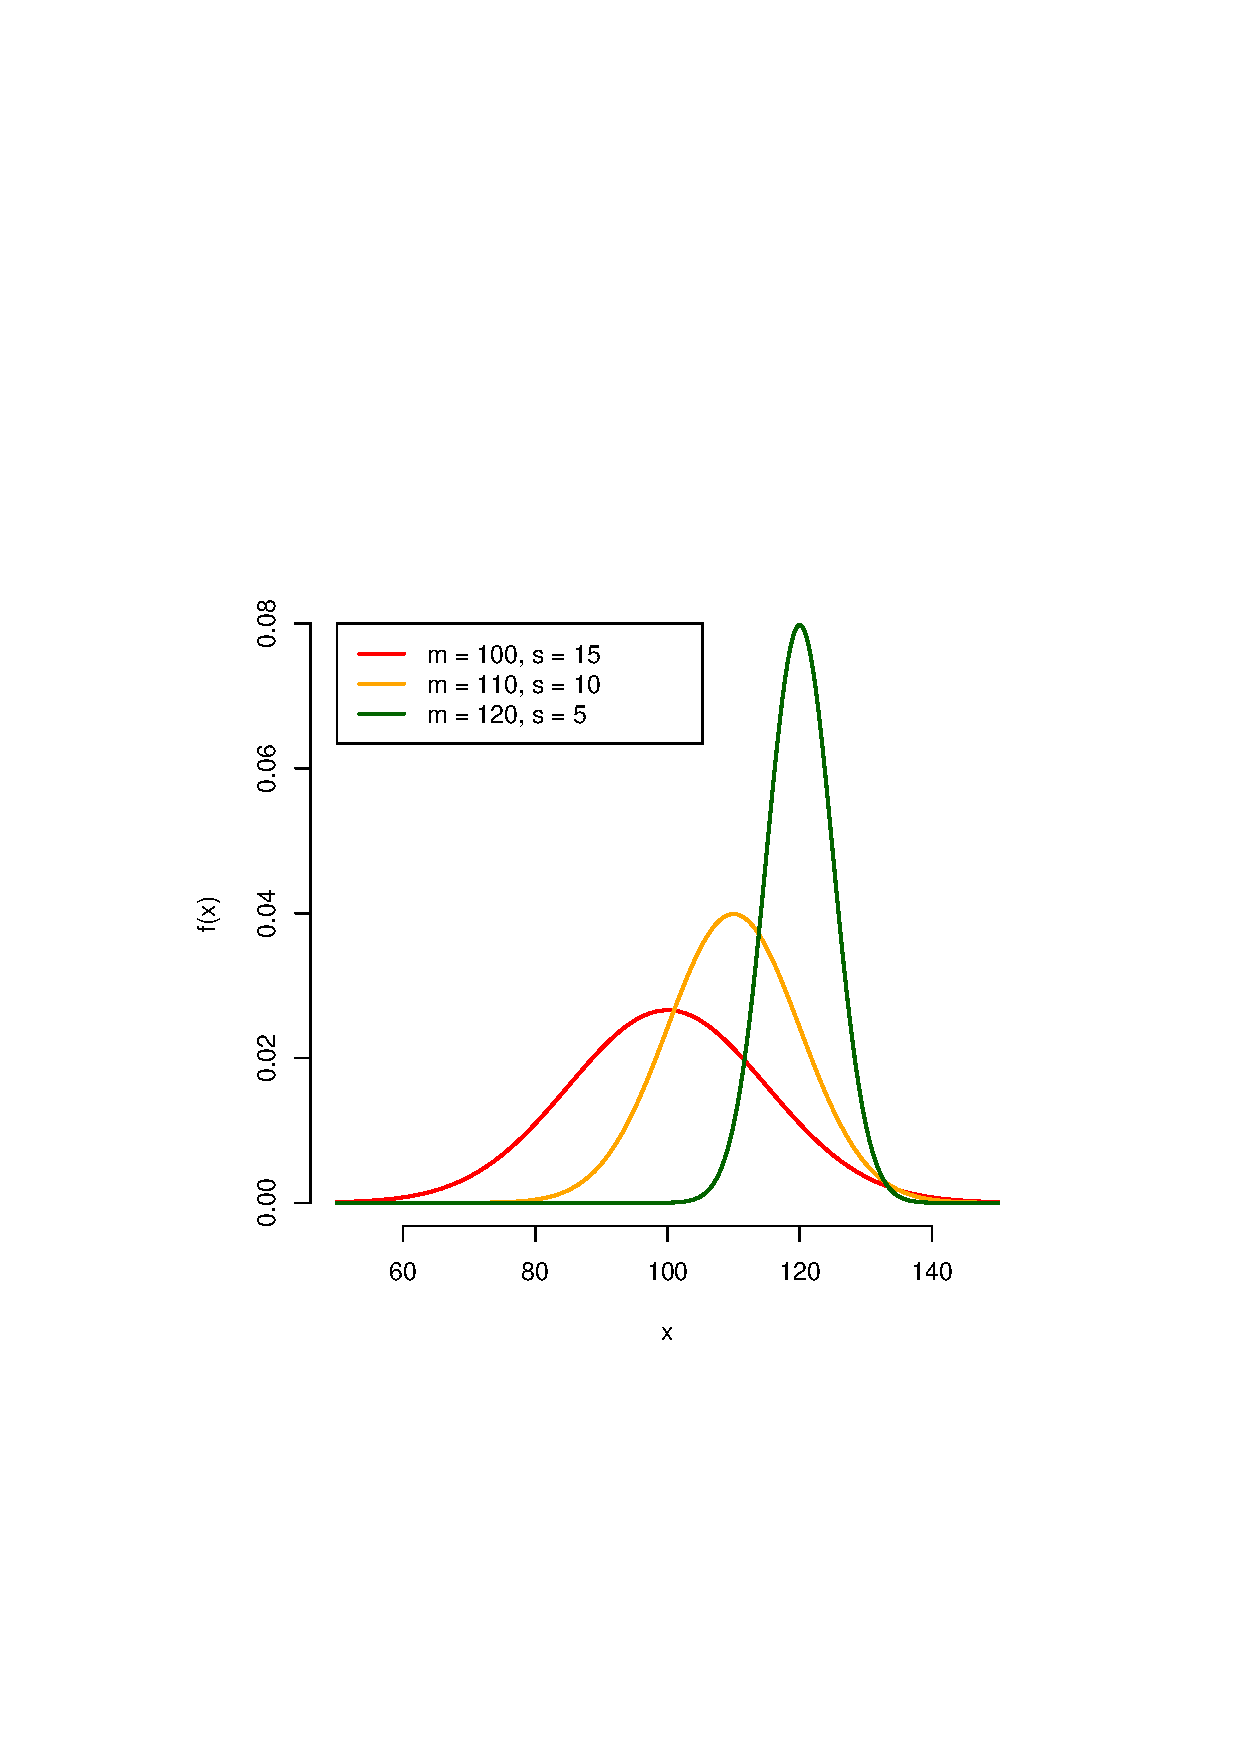
\includegraphics[width=6in, height=6in]{\FIGDIR/obr02}

\caption{Densities of several normal distributions.}
\label{obr03:Nhust}

\end{figure}


\begin{figure}[p]\centering
\psfrag{0.00}[c][c]{\textsf{\small 0{,}00}}  
\psfrag{0.02}[c][c]{\textsf{\small 0{,}02}}  
\psfrag{0.04}[c][c]{\textsf{\small 0{,}04}}
\psfrag{0.06}[c][c]{\textsf{\small 0{,}06}}  
\psfrag{0.08}[c][c]{\textsf{\small 0{,}08}}
\psfrag{60}[c][c]{\textsf{\small 60}}    
\psfrag{80}[c][c]{\textsf{\small 80}}  
\psfrag{100}[c][c]{\textsf{\small 100}}
\psfrag{120}[c][c]{\textsf{\small 120}}  
\psfrag{140}[c][c]{\textsf{\small 140}}
\psfrag{f\(x\)}[c][c]{\textsf{\small f(x)}}      
\psfrag{x}[c][c]{\textsf{\small x}}
\psfrag{m = 100, s = 15}[l][l]{\textsf{\large $\boldsymbol{\mu} \mathbf{\;= 100,}\; \boldsymbol{\sigma} \mathbf{\;= 15}$}}
\psfrag{m = 110, s = 10}[l][l]{\textsf{\large $\boldsymbol{\mu} \mathbf{\;= 110,}\; \boldsymbol{\sigma} \mathbf{\;= 10}$}}
\psfrag{m = 120, s = 5}[l][l]{\textsf{\large $\boldsymbol{\mu}  \mathbf{\;= 120,}\; \boldsymbol{\sigma} \mathbf{\;= 5}$}}

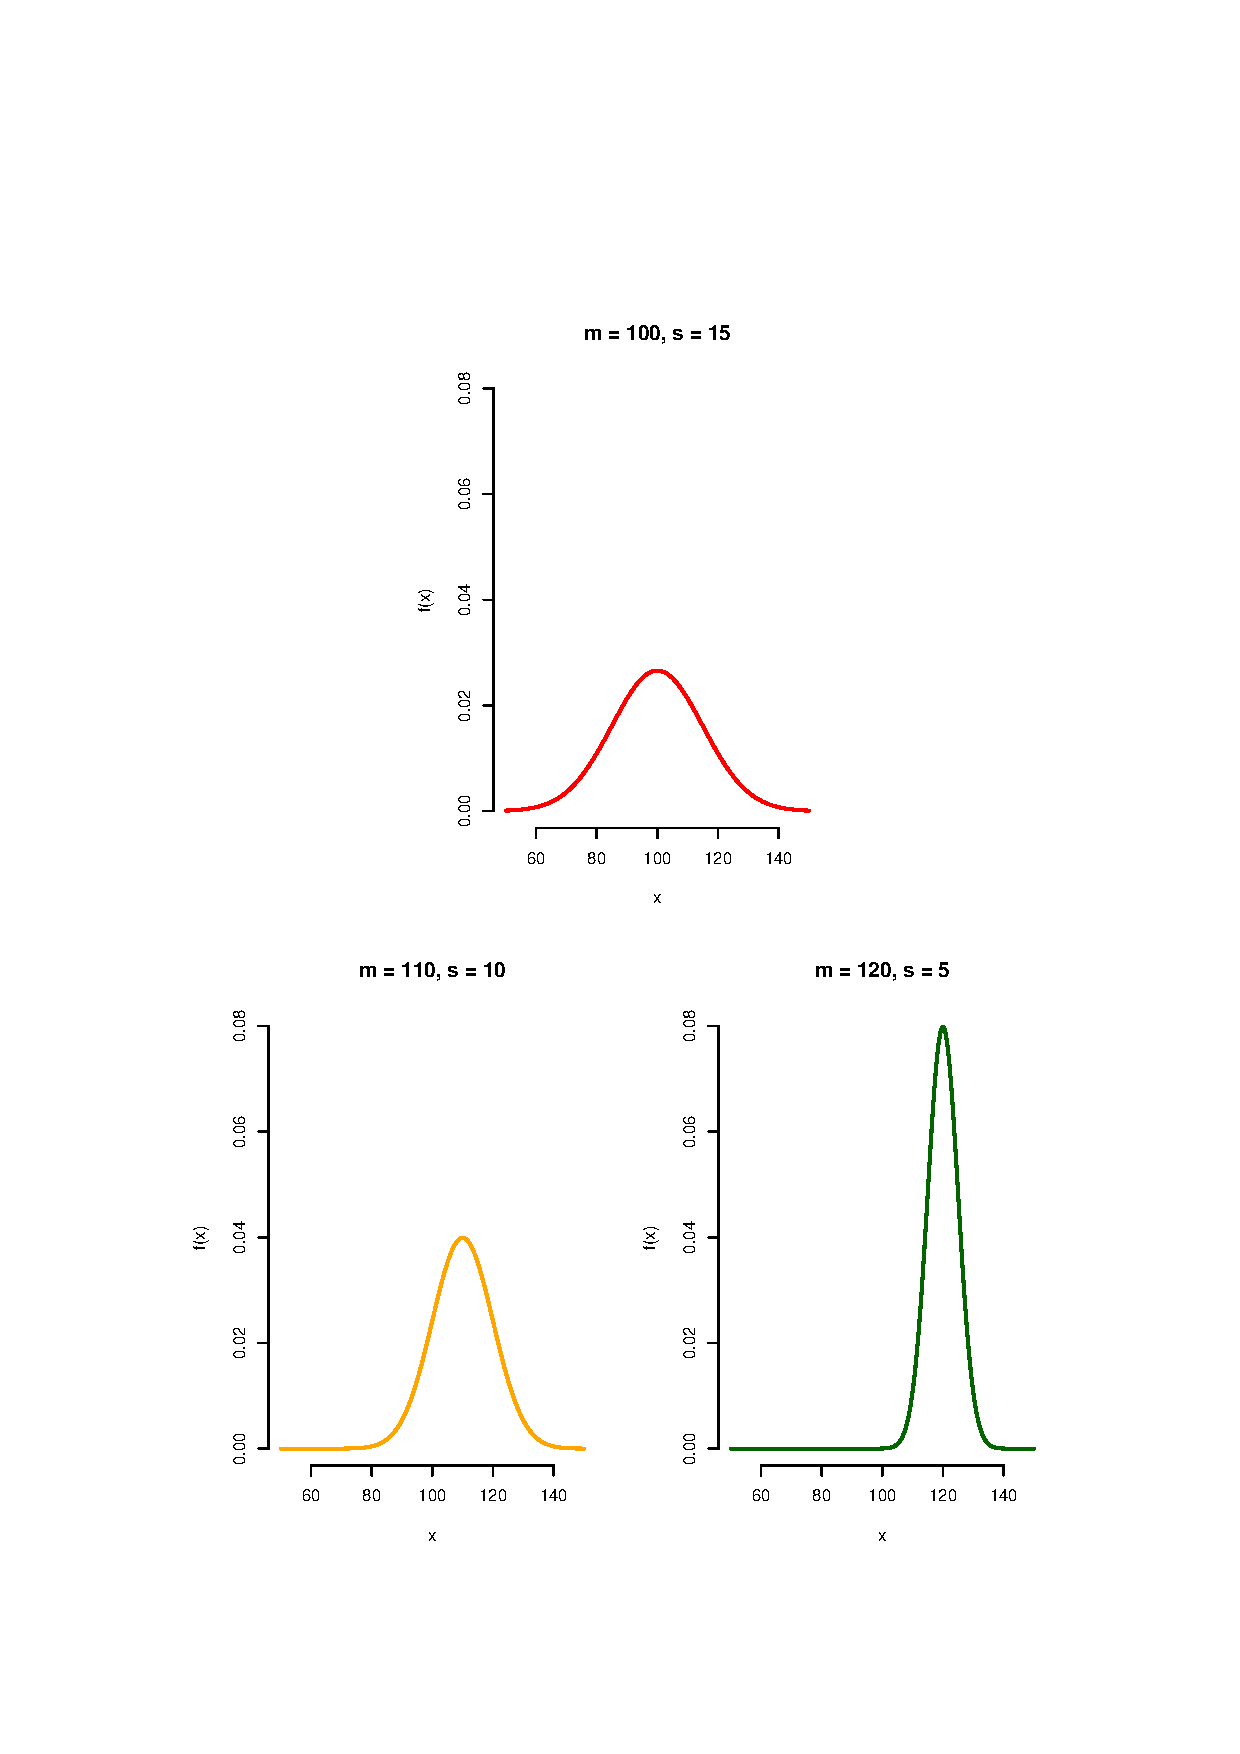
\includegraphics[width=6in, height=8.5in]{\FIGDIR/obr03}

\caption{Densities of several normal distributions.}
\label{obr03:Nhust:podruhe}

\end{figure}

